\documentclass{standalone}
\usepackage[T1]{fontenc}
\usepackage[latin2]{inputenc}
\usepackage[english]{babel}
\usepackage{tikz}
\usetikzlibrary{calc,through,backgrounds,positioning,fit}
\usetikzlibrary{shapes,arrows,shadows}
 
\begin{document}
 
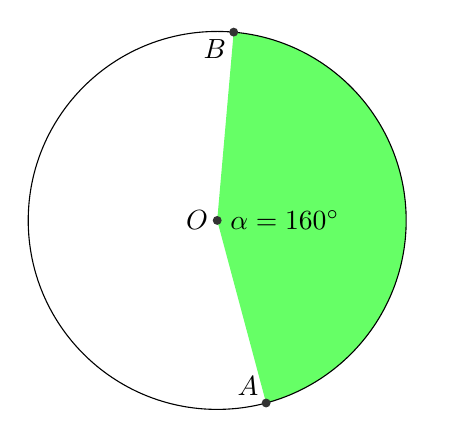
\begin{tikzpicture}[scale=1.2,inner sep=0.4mm]
\coordinate (O) at (0,0);
\coordinate (A) at (-75:2cm);
\coordinate (B) at (85:2cm);
\fill[green!60!white] (O) -- (A) arc (-75:85:2) -- cycle;
%\fill[green!60!white] (0,0) -- (1.4,0) arc (0:-80:1.4) -- cycle;
\node at (0.1,0) [right] {$\alpha=160^{\circ} $};
\draw(360:2) arc (360:0:2);
% ...
\node at (O) [circle,fill=black!80!white] {};
\node at (B) [below left=2pt] {$B$};
\node at (O) [left=2pt] {$O$};
\node at (A) [above left=2pt] {$A$};
\node at (A) [circle,fill=black!80!white] {};
\node at (B) [circle,fill=black!80!white] {};
\end{tikzpicture}
 
\end{document}